\documentclass[spanish,11pt,a4paper]{article}
\usepackage[margin=1in]{geometry}
\usepackage{fontspec}
\setmainfont{lmroman10-regular.otf}[BoldFont=lmroman10-bold.otf,ItalicFont=lmroman10-italic.otf,BoldItalicFont=lmroman10-bolditalic.otf]
\setsansfont{lmsans10-regular.otf}[BoldFont=lmsans10-bold.otf]
\setmonofont{lmmono10-regular.otf}[Scale=MatchLowercase]
\newlength{\LeanCharWidth}
\usepackage{amsmath,amssymb}
\usepackage[spanish,es-noshorthands]{babel}
\usepackage{microtype,parskip}
\usepackage{graphicx,float,caption}
\usepackage{longtable,booktabs,array,calc}
\usepackage{xcolor}
\usepackage{xurl}
\usepackage{hyperref,bookmark}
\usepackage{etoolbox,needspace}
\setcounter{secnumdepth}{-\maxdimen}
\setlength{\emergencystretch}{3em}
\providecommand{\tightlist}{\setlength{\itemsep}{0pt}\setlength{\parskip}{0pt}}
\newcounter{none}
\AtBeginEnvironment{longtable}{\Needspace{8\baselineskip}\small}
\pretocmd{\section}{\Needspace{5\baselineskip}}{}{}
\pretocmd{\subsection}{\Needspace{4\baselineskip}}{}{}
\pretocmd{\subsubsection}{\Needspace{4\baselineskip}}{}{}
\captionsetup{font=small,labelfont=bf}
\urlstyle{same}
\AtBeginDocument{\special{pdf:minorversion 7}}

\hypersetup{pdflang=es-CL,colorlinks=true,urlcolor=blue,linkcolor=blue,pdftitle={Recuperación de descomposiciones en triángulos con anfitrión tras borrados aleatorios en grafos split},pdfauthor={Juan Pablo Traverso Gianini}}
\title{Recuperación de descomposiciones en triángulos con anfitrión tras borrados aleatorios en grafos split}
\author{Juan Pablo Traverso Gianini\\\small Investigador independiente, Santiago, Chile\\\small\href{mailto:jtraverso@gmail.com}{jtraverso@gmail.com}\quad\href{https://orcid.org/0009-0003-6068-4096}{ORCID 0009-0003-6068-4096}}
\date{Preprint 1.0 \enspace·\enspace 24 de noviembre de 2026}
\begin{document}\raggedbottom\maketitle
\begin{center}Artículo III de la serie sobre brechas de partición en cliques en grafos split.\end{center}
\noindent DOI \url{https://doi.org/10.5281/zenodo.24494747}\\
Repositorio de la serie \url{https://github.com/jtraverso/split-clique-partition-gap}
\subsection{Resumen}\label{resumen}

Cada incidencia entre el núcleo y un anfitrión se conserva independientemente con probabilidad \(p\). Cuando los pares requeridos forman \(K_d\) o \(K_{d,d}\) y hay \(\lceil Kd\rceil\) anfitriones disponibles con \(Kp>1\), demostramos que, con alta probabilidad, las incidencias supervivientes contienen un soporte equilibrado que satisface las cuatro hipótesis de la absorción física tipada. Una sola descomposición de este soporte usa exactamente una vez cada par requerido y cada arista cruzada seleccionada.

Para todo \(0<p<1\) fijo y todo \(n\) suficientemente grande, la construcción da un grafo split de \(n\) vértices cuya brecha de partición en cliques, casi cuadrática, se conserva exactamente tras el borrado con alta probabilidad. En el mismo suceso, el grafo mantiene conectividad lineal por vértices. Una sola asignación aproxima las estadísticas lineales acotadas y los conteos de Pasch prescritos con error \(o(n^2)\) en todo el grafo y \(o(t^2)\) en los triángulos con base en el núcleo geométrico original de \(15t\) vértices. Los triángulos asignados a bases de ese núcleo contienen \((225p^2/8+o(1))t^2\) configuraciones de Pasch. Para grafos de solicitudes de grado máximo \(d\) y orden polinómico, la coloración ponderada de aristas por listas da la condición uniforme óptima \(Kp>1\) para recuperar la asignación con \(\lceil Kd\rceil\) anfitriones.

\subsection{1. Reconstrucción, estadísticas prescritas y brecha de partición en cliques}\label{reconstrucciuxf3n-estaduxedsticas-prescritas-y-brecha-de-particiuxf3n-en-cliques}

En un grafo split, los vértices del núcleo forman una clique y los demás un conjunto independiente. Toda clique que corta el conjunto independiente contiene un único vértice de ese conjunto, al que llamamos su \emph{anfitrión}. La Parte I, \emph{Nearly Quadratic Additive Gaps for Edge-Clique Partitions of Split Graphs} {[}1{]}, utilizó triángulos con anfitrión para realizar un problema de empaquetamiento en el núcleo. La Parte II, \emph{Stability of the Clique Partition Gap in Split Graphs} {[}2{]}, mostró que al perder \(L\) asignaciones la comparación con dicho problema cambia en a lo sumo \(2L\). La construcción que allí permitía una cantidad cuadrática de borrados protegía los triángulos asignados sobre el núcleo original. Aquí pueden borrarse ambas aristas cruzadas de cada triángulo asignado. Cuando un par pierde su triángulo, quizá conserve otro anfitrión común. Para recuperar todos los pares a la vez, los triángulos de reemplazo deben usar aristas cruzadas distintas.

Una \emph{base} es un par requerido de vértices del núcleo. Al asignarla a un anfitrión común se obtiene un triángulo cuyas dos aristas cruzadas unen sus extremos con ese anfitrión. La asignación es \emph{propia} si las bases asignadas a cada anfitrión forman un emparejamiento. En nuestra construcción, toda asignación propia completa conserva la brecha de partición en cliques. La prescripción de estadísticas también restringe la elección de triángulos. Una configuración de Pasch consta de cuatro triángulos sobre seis vértices, cada vértice aparece dos veces y los triángulos son disjuntos en aristas.

Sea \(\operatorname{cp}(G)\) el número mínimo de cliques en una partición de las aristas de \(G\). Su versión fraccionaria \(\operatorname{cp}^{\ast}(G)\) minimiza la suma de pesos no negativos sobre las cliques, con peso total uno en cada arista. Se admiten cliques de cualquier orden a partir de dos. Escribimos \(\Delta(G)=\operatorname{cp}(G)-\operatorname{cp}^{\ast}(G)\) y denotamos por \(\kappa(G)\) la conectividad por vértices. En lo que sigue, \(p\) denota la probabilidad de que una arista cruzada \emph{sobreviva}. Se conservan todas las aristas del núcleo. Los logaritmos son naturales.

\textbf{Teorema 1 (reconstrucción de un soporte equilibrado).} Fijemos \(0<p<1\) y \(K>1/p\). Existen constantes \(C\ge1\), \(\alpha>0\) y \(\eta_0>0\), con \(\eta_0<Kp-1\), para las que vale lo siguiente. Para cada \(0<\eta<\eta_0\) fijo existen \(c>0\) y \(d_0\) tales que, si \(d\ge d_0\), podemos partir de \(K_{d,d}\) o \(K_d\) como grafo de bases y designar antes del borrado cualesquiera \(r=\lceil(1+\eta)d/p\rceil\) de los \(\lceil Kd\rceil\) anfitriones disponibles. Cada incidencia cruzada se conserva independientemente con probabilidad \(p\). Con probabilidad al menos \(1-\exp(-c d^{1/3})\) existe un grafo \(H\) sobre el núcleo y estos \(r\) anfitriones cuyas aristas son todas las bases y un subconjunto de las aristas cruzadas supervivientes. Escribimos \(N=|V(H)|\). Los tipos de triángulo permitidos son (izquierda, derecha, anfitrión) en el caso bipartito y (núcleo, núcleo, anfitrión) en el caso de la clique. En ese mismo \(H\) se cumplen las cuatro propiedades siguientes.

\begin{enumerate}
\def\labelenumi{\arabic{enumi}.}
\tightlist
\item
  \textbf{Semilla difusa (H1).} Cada triángulo permitido \(T\) tiene un peso \(\mu_T\in[1/(CN),C/N]\) y los pesos en cada arista de \(H\) suman uno.
\item
  \textbf{Certificado entero (H2).} El vector indicador de aristas de \(H\) es una combinación lineal entera de los vectores indicadores de sus triángulos permitidos.
\item
  \textbf{Vecinos comunes (H3).} Para cada par de vértices distintos y cada etiqueta que completa sus etiquetas a un tipo permitido, al menos \(\alpha N\) vecinos comunes tienen esa etiqueta. Esto incluye los pares sin arista.
\item
  \textbf{Bisagras físicas (H4).} Para los triángulos permitidos \(uvx,uvy\) con \(x\ne y\), existen al menos \(\alpha N^2\) conjuntos distintos de aristas auxiliares \(J\subseteq E(H)\), incidentes con exactamente seis vértices y disjuntos en aristas de ambos triángulos raíz. Tanto \(J\cup\{ux,vx\}\) como \(J\cup\{uy,vy\}\) admiten una descomposición en triángulos permitidos.
\end{enumerate}

Para una reserva inicial de \(r\) anfitriones de la base \(e\), damos a cada uno de sus \(r\) triángulos candidatos el peso \(\lambda_T=1/r\). Estos pesos representan la elección uniforme de un anfitrión para cada base antes de conocer qué incidencias sobreviven. Sea \(\mathcal C\) el conjunto de candidatos, restringido a la reserva designada para cada base. Para una función de prueba real \(f\) sobre \(\mathcal C\) y el conjunto \(\mathcal P(\mathcal C)\) de sus configuraciones de Pasch no ordenadas, los dos valores objetivo son

\[M_\lambda(f)=\sum_{T\in\mathcal C} f(T)\lambda_T,\qquad
P_\lambda=\sum_{P\in\mathcal P(\mathcal C)}\prod_{T\in P}\lambda_T.
\tag{1}\]

Por ejemplo, si \(f\) es el indicador de los triángulos que usan un conjunto dado de anfitriones, se mide su contribución a la asignación final. La fórmula (1) admite también funciones de prueba con signo.

\textbf{Teorema 2 (estadísticas a dos escalas).} Para \(0<p<1\) fijo existe una sucesión de grafos split de cada orden \(n\) suficientemente grande que satisface el Teorema 3. Cada grafo posee un núcleo original \(U\) de \(15t\) vértices, con \(t=\Theta_p(n/\sqrt{\log n})\), y reservas iniciales de anfitriones elegidas antes del borrado. La misma sucesión y sus reservas sirven para todo \(q\ge0\) fijo. Dada una familia \(\mathcal F_n\) de a lo sumo \(n^q\) funciones de prueba \(|f|\le1\) elegidas antes del borrado, con probabilidad que tiende a uno existe una asignación propia completa \(\mathcal D\) en el grafo superviviente tal que \[\max_{f\in\mathcal F_n}\left|\sum_{T\in\mathcal D}f(T)-M_\lambda(f)\right|=o(n^2),
\qquad |P(\mathcal D)-P_\lambda|=o(n^2).
\tag{2}\]

Denotamos por \(\mathcal D_U\) y \(\mathcal C_U\) los triángulos asignados y los candidatos, respectivamente, cuyos dos vértices del núcleo están en \(U\). Con los pesos de (1), restringidos a \(\mathcal C_U\), definimos \(M_{\lambda,U}\) y \(P_{\lambda,U}\). La misma asignación satisface \[\max_{f\in\mathcal F_n}\left|\sum_{T\in\mathcal D_U}f(T)-M_{\lambda,U}(f)\right|=o(t^2),
\qquad |P(\mathcal D_U)-P_{\lambda,U}|=o(t^2).
\tag{3}\]

Para la familia vacía, las cotas sobre las funciones de prueba son vacuas. Cada base y cada arista cruzada del soporte seleccionado pertenece a exactamente un triángulo de \(\mathcal D\). Con \(|W|\sim p^2n/64\) vértices adicionales en el núcleo, los dos conteos son \[P(\mathcal D)=\frac{p^6}{32768}\,n^2+o(n^2),
\qquad
P(\mathcal D_U)=\frac{225p^2}{8}\,t^2+o(t^2).
\tag{4}\]

\textbf{Teorema 3 (brecha y conectividad).} Fijemos \(0<p<1\). Existen constantes \(a_p,c_p>0\) tales que para todo \(n\) suficientemente grande hay un grafo split \(G_n\) de \(n\) vértices con

\[\Delta(G_n)\ \ge\ a_p\,\frac{n^2}{(\log n)^{5/2}}
  \exp\!\left(-2\sqrt{\log(24/7)\log n}\right).
\tag{5}\]

Sea \(G'_n\) el grafo obtenido al conservar cada arista cruzada independientemente con probabilidad \(p\). Entonces

\[\Pr\!\left(\Delta(G'_n)=\Delta(G_n)
             \ \text{and}\ \kappa(G'_n)\ge c_p n\right)\longrightarrow 1.
\tag{6}\]

Balogh, He, Krueger, Nguyen y Wigal {[}7, Teorema 1.10{]} obtienen \(\Delta(G)=o(n^2)\) para grafos generales tomando \(t=2\) y asignando costes unitarios a las cliques en su teorema de descomposición. Dentro de este régimen subcuadrático, la cota inferior (5) es de orden \(n^{2-o(1)}\). Para un triángulo dado antes del borrado, la probabilidad de que sobrevivan ambas aristas cruzadas es \(p^2\). Bajo la condición de independencia de las vecindades que se enuncia abajo, toda asignación propia completa de los mismos pares requeridos realiza la misma brecha de empaquetamiento. Recordamos el enunciado preciso de {[}1, Lema 2.1{]} y {[}2, Lema 2{]}.

Sea \(V\) el núcleo y sea \(B\) un grafo sobre \(V\), al que llamamos \emph{grafo residual}. Los pares requeridos son \(J=\binom V2\setminus E(B)\). Para un conjunto \(Q\) del núcleo de orden al menos dos, su puntuación residual es

\[w_B(Q)=\binom{|Q|}{2}-1-2\left|J\cap\binom Q2\right|.\]

Los dos primeros términos expresan el ahorro de usar \(Q\) como clique respecto de sus aristas individuales. Cada par requerido que ocupa \(Q\) desplaza un posible triángulo con anfitrión, cuyo ahorro es dos. Sea \(I(B)\) la puntuación total máxima sobre familias de conjuntos del núcleo que usan cada par a lo sumo una vez. El máximo fraccionario \(F(B)\) permite un peso no negativo para cada conjunto e impone la misma capacidad unitaria en cada par. Ponemos \(\Phi(B)=F(B)-I(B)\).

Los triángulos de una asignación propia a anfitriones son disjuntos en aristas. Si cada vecindad de anfitrión es independiente en \(B\) y existe una asignación propia de todo \(J\), las identidades de transferencia exacta dan

\[\operatorname{cp}(G)=|E(G)|-2|J|-I(B),\qquad
\operatorname{cp}^{\ast}(G)=|E(G)|-2|J|-F(B).
\tag{7}\]

Al restar se cancela el término que contiene \(|E(G)|\). Los borrados pueden reducir una vecindad de anfitrión y preservan su independencia en \(B\). Por tanto, para recuperar la brecha basta asignar de nuevo los mismos pares requeridos. La sección 2 demuestra la recuperación para una reserva de anfitriones. En las secciones 3 y 4 asignamos un bloque a cada par requerido de la Parte I. En las secciones 5 y 6 reconstruimos el soporte equilibrado y controlamos las estadísticas de una sola descomposición a ambas escalas.

\subsection{2. Recuperación a partir de listas aleatorias de anfitriones}\label{recuperaciuxf3n-a-partir-de-listas-aleatorias-de-anfitriones}

Sea \(R\) un grafo simple finito de solicitudes. Al principio cada anfitrión es vecino de todos los vértices de \(R\). Tras el borrado, la lista de cada arista \(uv\) de \(R\) contiene los anfitriones que siguen siendo vecinos tanto de \(u\) como de \(v\). Estas listas son dependientes. Por ejemplo, perder la incidencia \(hu\) retira a \(h\) de todas las listas en \(u\). El siguiente resultado usa este modelo de incidencias. Escribimos \(d\) para el grado máximo de \(R\), a fin de distinguirlo de la brecha de partición.

\textbf{Teorema 4 (recuperación a partir de listas aleatorias de anfitriones).} Fijemos \(p\in(0,1)\), \(K>1/p\) y \(A\ge1\). Supongamos que \(R\) tiene grado máximo \(d\) y a lo sumo \((d+1)^A\) vértices. Dotamos a \(R\) de \(\lceil Kd\rceil\) anfitriones y conservamos cada incidencia vértice--anfitrión independientemente con probabilidad \(p\). Para todo \(d\) suficientemente grande, existe una asignación propia de todas las aristas de \(R\) salvo en un suceso de probabilidad a lo sumo \(C d^{C}\exp(-c\sqrt d)\), para constantes \(C,c>0\) que dependen solo de \(p,K,A\). Para \(K>0\) con \(Kp\le1\), la conclusión uniforme con alta probabilidad falla incluso para \(K_{d+1}\), que pertenece a la clase de tamaños indicada para todo \(A\ge1\).

\emph{Demostración.} Un vértice de grado \(d\) necesita al menos \(d\) anfitriones distintos. Si \(Kp<1\), el número de anfitriones que conserva es una variable binomial de media a lo sumo \(Kpd+1\) y queda por debajo del mínimo con probabilidad que tiende a uno. Cuando \(Kp=1\), el grafo completo \(R=K_{d+1}\) proporciona la obstrucción. Cada vértice conserva un número binomial de anfitriones, de media \(d+O(1)\) y varianza de orden \(d\). Por el teorema central del límite, la probabilidad de que conserve menos de \(d\) tiende a \(1/2\). Los conteos de vértices distintos usan incidencias disjuntas. Con probabilidad que tiende a uno, algún vértice queda por debajo del mínimo.

Supongamos ahora \(Kp>1\) y pongamos \(m=\lceil Kd\rceil\). Para una solicitud \(e=uv\), sea \(L(e)\) su lista superviviente, y sea \(Z(u,h)\) el número de solicitudes en \(u\) cuya lista contiene a \(h\). El tamaño de la lista tiene distribución \(\mathrm{Bin}(m,p^2)\). Condicionado a que \(hu\) sobreviva, \(Z(u,h)\) tiene distribución \(\mathrm{Bin}(\deg_R(u),p)\) porque los otros extremos de esas solicitudes son distintos. En caso contrario, \(Z(u,h)=0\). La desigualdad de Chernoff y una cota de unión sobre a lo sumo \(d(d+1)^A/2\) solicitudes y \(m(d+1)^A\) incidencias dan, simultáneamente, \[|L(e)|\ge mp^2-d^{3/4},\qquad Z(u,h)\le pd+d^{3/4}
 \tag{8}\] salvo con probabilidad \(d^{O(1)}\exp(-\Omega_{p,K}(\sqrt d))\).

Ponemos \(b=\lceil pd+d^{3/4}\rceil\) y damos a cada color de anfitrión disponible un peso \(1/b\). En un extremo \(u\), las aristas que compiten por un color \(h\) tienen peso total a lo sumo \(Z(u,h)/b\le1\). Cada lista tiene peso total al menos \((mp^2-d^{3/4})/b\), que tiende a \(Kp\). Para \(d\) grande, es al menos \(1+(Kp-1)/2\). Los pesos individuales satisfacen \(\exp(-b^{1/25})\le1/b\). Estas son las cotas de peso, masa de lista y conflicto del teorema de Bonamy, Delcourt, Lang y Postle {[}3, Teorema 6{]}, aplicado con parámetro \(b\) al grafo simple \(R\). Una coloración propia de aristas por listas da la asignación requerida en el suceso (8). \(\square\)

En los modelos de listas aleatorias estudiados por Jain y Pham {[}8{]} y Keevash {[}10{]}, el muestreo de colores se hace para las aristas del grafo de solicitudes. En nuestro modelo, los ensayos independientes son las incidencias vértice--anfitrión. La pérdida de \(hu\) retira a \(h\) de todas las listas en \(u\) a la vez. Condicionar a la supervivencia de \(hu\) da la cota local de conflictos requerida por el teorema de coloración.

\subsection{3. Una reserva de anfitriones para cada par requerido del núcleo}\label{una-reserva-de-anfitriones-para-cada-par-requerido-del-nuxfacleo}

Usamos los siguientes datos de la construcción de {[}1, §§4--6{]}. Sus quince roles se agrupan en tres clases de color, con cinco roles por clase. En cada rol, las posiciones son los elementos de

\[D_m=(\mathbb Z/m\mathbb Z)^2,\qquad T=D_m^j,\qquad t=|T|=m^{2j},\]

donde \(m\) es impar y \(j\ge2\). De los pares de roles, contando una vez cada rol repetido, 54 son aristas del grafo de quince roles. Para uno de esos pares, sea \(b\in\{1,2\}\) la diferencia de sus índices de color en orden creciente. El par del núcleo con posiciones \(x,y\) es arista de \(B\) si y solo si su dirección \((y-x)/b\) está en \(S_m^j\), donde \(S_m\subset D_m\) es el conjunto de {[}1{]}. Para cada uno de los 66 tipos de rol restantes se requieren todos los pares de vértices distintos. Para construir los anfitriones usamos una sola propiedad geométrica de \(S_m\). Su complemento se puede partir en a lo sumo 24 clases \(C\) tales que

\[u,v\in C\quad\Longrightarrow\quad (u+v)/2\notin S_m.
\tag{9}\]

La división por dos está bien definida porque \(m\) es impar. La cota cuantitativa de empaquetamiento para este \(S_m\) se usa en la sección 4.

Para contar los anfitriones disponibles para un par, fijamos un conjunto de direcciones \(U\subset T\) y un centro \(z\in T\). Un anfitrión es vecino de las posiciones \(z-bU/2\) en el primer rol y \(z+bU/2\) en el segundo. Para el par \((x,x+ba)\) de dirección \(a\), ponemos \(u=2(z-x)/b\). La primera condición de pertenencia es \(u\in U\) y la segunda, \(x+ba\in z+bU/2\), equivale a \(2a-u\in U\). El número de centros que sirven a este par es exactamente \(|U\cap(2a-U)|\). Especificar una clase hasta la última coordenada puede dejar muy pocos centros. Si una coordenada queda libre, al variarla en el centro se obtienen al menos \(m^2\) opciones intercambiables para cada par designado a la clase.

\textbf{Lema 5 (dos órdenes de las coordenadas).} Para todo entero \(K\ge1\), los pares requeridos en los 54 tipos de rol admiten un sistema de a lo sumo \(1296Kjt\) anfitriones con vecindades independientes en \(B\). Cada par requerido se designa a un solo grafo bipartito completo auxiliar \(K_{d,d}\) con \(d\ge m^2\) y \(Kd\) anfitriones disponibles. Dos grafos auxiliares que usan los mismos anfitriones tienen conjuntos de vértices disjuntos. Al restringir cada asignación a los pares designados a su bloque, las asignaciones propias de todos los grafos auxiliares dan una asignación propia de todos los pares requeridos de estos tipos.

\emph{Demostración.} \emph{Asignación de cada dirección a un bloque.} En el orden \(1,\ldots,j\) usamos la primera coordenada fuera de \(S_m\) cuando aparece entre las primeras \(j-1\). Si todas ellas pertenecen a \(S_m\), la última queda necesariamente fuera. En ese caso leemos las coordenadas en el orden \(1,\ldots,j-2,j,j-1\). A la coordenada que falla le sigue ahora la penúltima del orden original. Por ejemplo, con tres coordenadas, una dirección en \(S_m\times S_m\times C\) se trata en el orden \(1,3,2\) y deja libre la coordenada 2. Las dos reglas asignan cada dirección requerida exactamente una vez.

\[\begin{array}{c|ccc|c}
 &\text{prefijo común}&\text{coordenada siguiente}&\text{coordenada libre}&\text{tamaño del bloque}\\ \hline
 \text{primario}&1,\ldots,j-2&j-1\ \text{falla}&j&K_{m^2,m^2}\\
 \text{secundario}&1,\ldots,j-2&j\ \text{falla}&j-1&K_{m^2,m^2}
\end{array}\]

\emph{Tabla 1. Los dos órdenes cuando las primeras \(j-2\) coordenadas satisfacen la condición. Una dirección se asigna al bloque secundario solo si su coordenada original \(j-1\) también la satisface. En el bloque auxiliar completo esa coordenada varía libremente antes de restringir a las bases que le corresponden.}

Para una coordenada que falla en cualquiera de los dos órdenes, escribimos \(U=S_m^\ell\times C\times D_m^{j-\ell-1}\) respecto de ese orden, donde \(\ell\) coordenadas preceden al fallo. Para cada centro \(z\) tomamos \(K\) anfitriones con las dos vecindades anteriores. La dirección entre dos vecinos cualesquiera de roles opuestos es el punto medio de dos elementos de \(U\). Por (9) queda fuera de \(S_m^j\). Los vértices de un mismo rol son independientes en \(B\), así que toda la vecindad es independiente.

\emph{El bloque bipartito completo.} Fijamos el prefijo del centro hasta la coordenada que falla, incluida esta. Las \(d=m^{2(j-\ell-1)}\) opciones del sufijo dan vecindades idénticas. Por tanto, disponemos de \(Kd\) anfitriones comunes. Para una dirección del prefijo \(u\), los prefijos de los extremos emparejados son \(z-bu/2\) y \(z+bu/2\), con todas estas cantidades restringidas al prefijo. Cualquiera de los dos extremos determina al otro por reflexión respecto de \(z\). Pares distintos de estos prefijos tienen, por tanto, extremos disjuntos. Por encima de cada par de prefijos, los dos sufijos varían libre e independientemente y forman un \(K_{d,d}\) completo. Cada par designado determina el prefijo de su centro mediante el punto medio de sus extremos.

\emph{Reutilización de una reserva.} En el segundo orden, el grafo bipartito completo contiene algunos pares cuya penúltima coordenada original ya fallaba. Esos pares corresponden al primer orden. Podemos colorear el grafo auxiliar entero y retirar luego los triángulos de los pares asignados a otro bloque. A cada par que queda le corresponde un único bloque. Como los prefijos son disjuntos, se puede volver a usar un anfitrión sin repetir una incidencia. Hay a lo sumo \(24(j-1)\) plantillas en el primer orden y 24 en el segundo, cada una con \(Kt\) anfitriones por tipo de rol. Al multiplicar por 54 se obtiene la cota anunciada. \(\square\)

\subsection{4. Demostración del Teorema 3}\label{demostraciuxf3n-del-teorema-3}

Elegimos un entero \(K>1/p\). Describimos los demás anfitriones antes de fijar \(m\) y \(j\), pues su número determina el tamaño del núcleo que cabe en un grafo de orden \(n\). Añadimos a la clique un conjunto \(W\) de \(x\) vértices, todos aislados en el residual. Cada anfitrión será vecino de todo \(W\) antes del borrado. Además de los anfitriones del Lema 5, bastan diez reservas. Las siete ternas de la tabla son los siete triángulos disjuntos en aristas que se retiran del grafo tripartito de roles en {[}1{]}. Se requieren los tres pares de roles de cada terna.

{\def\LTcaptype{none} % do not increment counter
\begin{longtable}[]{@{}
  >{\raggedright\arraybackslash}p{(\linewidth - 4\tabcolsep) * \real{0.3000}}
  >{\raggedleft\arraybackslash}p{(\linewidth - 4\tabcolsep) * \real{0.4000}}
  >{\raggedright\arraybackslash}p{(\linewidth - 4\tabcolsep) * \real{0.3000}}@{}}
\toprule\noalign{}
\begin{minipage}[b]{\linewidth}\raggedright
Reserva de anfitriones
\end{minipage} & \begin{minipage}[b]{\linewidth}\raggedleft
Anfitriones por reserva
\end{minipage} & \begin{minipage}[b]{\linewidth}\raggedright
Solicitudes coloreadas antes de restringir
\end{minipage} \\
\midrule\noalign{}
\endhead
\bottomrule\noalign{}
\endlastfoot
Una por cada clase de color \(V_i\) & \(K(x+5t)\) & Todos los pares de \(W\cup V_i\) \\
Una por cada una de las siete ternas de roles retiradas & \(2Kt\) & El grafo tripartito completo sobre sus tres roles, cada uno de tamaño \(t\) \\
\end{longtable}
}

Las tres primeras reservas son vecinas de \(W\cup V_i\). Cubren todos los pares internos de una clase de color y todos los pares de \(W\) con esa clase. Conservamos la asignación dentro de \(W\) solo en la primera reserva. Cada una de las otras siete reservas es vecina de sus tres roles y de \(W\). Se encarga de los tres pares de roles distintos de su terna. Estos 21 tipos entre colores y los 45 tipos de un mismo color comprenden los 66 tipos de rol restantes. Cada vecindad es independiente en el residual ampliado. Las diez reservas suman \(3Kx+(15+14)Kt\) anfitriones.

Ponemos \(\gamma=\log(24/7)\) y definimos

\[j=\left\lfloor\sqrt{\log n/\gamma}\right\rfloor,\quad
B_j=15+(1296j+29)K,\quad
x=\left\lfloor\frac{n}{2(1+3K)}\right\rfloor.\]

Tomamos el mayor impar positivo \(m\) que satisface \(B_jm^{2j}\le n/4\), usando el parámetro \(7/(1080j)\) de {[}1{]} en la definición de \(S_m\). El núcleo original, los anfitriones del Lema 5, las diez reservas adicionales y \(W\) suman a lo sumo

\[B_jt+(1+3K)x\le 3n/4\]

vértices. Al dar a cada vértice restante la vecindad \(W\), el orden queda exactamente en \(n\).

Para estos parámetros, \(t=\Theta_p(n/j)\). En efecto, para \(X=(n/(4B_j))^{1/(2j)}\) tenemos \(X-2<m\le X\) y \(\log X=\Theta(\sqrt{\log n})\). Por tanto, \(j/X\to0\), y al elevar \(m/X\) a la potencia \(2j\) resulta \(1-o(1)\). La estimación residual de la Parte I {[}1, §§4--6{]}, cuya constante implícita es absoluta, da

\[\begin{aligned}
\Phi(B)&\gg \frac{(7/24)^j t^2}{j^3m^2}\\
&\gg_p \frac{n^2}{j^5}\exp(-\gamma j-\log n/j).
\end{aligned}
\tag{10}\]

En la segunda línea usamos \(m^2=t^{1/j}\le n^{1/j}\). Para \(y=\sqrt{\log n/\gamma}\) tenemos \(0\le y-j<1\), por lo que \(\gamma j+\log n/j=2\gamma y+\gamma(j-y)^2/j\). Esto demuestra la estimación (5) para \(\Phi(B)\).

Consideramos ahora las incidencias supervivientes. Cada grafo bipartito del Lema 5 tiene \(2d\) vértices, grado máximo \(d\ge m^2\) y \(Kd\) anfitriones disponibles. Se puede aplicar el Teorema 4. Contando con multiplicidad las bases de los grafos auxiliares completos obtenemos a lo sumo \(108t^2\) bases, ya que cada par de roles y cada par de posiciones aparecen a lo sumo una vez por orden. Esa cota también limita el número de bloques no vacíos. Para \(m\) suficientemente grande, la cota de fallo del Teorema 4 en cada bloque es a lo sumo \(\exp(-c'm)\) para algún \(c'>0\). Como \(m/\log n\to\infty\), la suma de estas probabilidades tiende a cero.

En cada una de las tres reservas de color, el grafo completo tiene grado \(x+5t-1\). En cada una de las siete reservas de ternas, el grado es \(2t\). En ambos casos, la tabla ofrece al menos \(K\) veces el grado en anfitriones. El mismo teorema se aplica a cada uno de esos diez grafos. Por tanto, con probabilidad que tiende a uno existe una asignación completa tras aplicar las restricciones del Lema 5 y retirar las dos asignaciones duplicadas dentro de \(W\). La cota de unión permite tratar conjuntamente los fallos de todos los bloques.

El residual ampliado es \(B^+=B\sqcup I_W\), donde \(I_W\) es el grafo vacío sobre \(W\). La Parte I {[}1, §6{]} da \(\Phi(B^+)=\Phi(B)\). Para \(n\) suficientemente grande, la probabilidad de éxito es positiva. Cada triángulo de una asignación exitosa está presente en \(G_n\), así que esa asignación sirve también antes del borrado. Aplicando (7) a los dos grafos en cada realización exitosa, obtenemos

\[\Delta(G'_n)=\Phi(B^+)=\Phi(B)=\Delta(G_n).\]

Por último, el número de vecinos que cada anfitrión conserva en \(W\) tiene distribución \(\mathrm{Bin}(x,p)\) y media \(px\). La probabilidad de que algún anfitrión conserve menos de \(px/2\) es a lo sumo \(ne^{-px/8}=o(1)\). Al retirar menos de \(px/2\) vértices queda una clique no vacía en el núcleo y cada anfitrión restante conserva un vecino en ella. Como \(x=\Theta_p(n)\), se sigue la afirmación de conectividad de (6). Hay una cantidad lineal de anfitriones y de vértices en \(W\), de modo que se borran \(\Theta_p(n^2)\) aristas cruzadas con probabilidad que tiende a uno. \(\square\)

\subsubsection{Una comparación determinista}\label{una-comparaciuxf3n-determinista}

El modelo aleatorio permite pérdidas en cada vértice. Para pérdidas adversarias podemos dar un cupo por vértice, usando los parámetros de tamaño originales de la Parte I. La comparación también indica en qué paso del Teorema 3 interviene la independencia.

\textbf{Proposición 6.} Con los parámetros \(m,j,n\) de {[}1, §6{]}, sean \(s=m^{2j-2}\), \(v=15m^{2j}\), \(w=\lceil n/5\rceil\) y \(r=\lfloor n/100\rfloor\). Para todo \(n\) suficientemente grande se pueden elegir anfitriones al mismo orden y con la misma brecha residual que en {[}1{]}, de modo que se cumplan simultáneamente los dos cupos siguientes. En cualquier vértice del núcleo original pueden borrarse hasta \(\lfloor s/2\rfloor\) incidencias en cada uno de los grupos originales de anfitriones que se le designaron. En cualquier vértice del núcleo ampliado pueden borrarse además hasta \(\lfloor(v+r)/2\rfloor\) incidencias en la unión de las tres familias de relleno. El grafo superviviente conserva la brecha original.

La demostración está en el apéndice A.

\subsection{5. Reconstrucción de un soporte para la absorción física tipada}\label{reconstrucciuxf3n-de-un-soporte-para-la-absorciuxf3n-fuxedsica-tipada}

Una asignación completa usa un emparejamiento en cada anfitrión. Esto fija cuántos pares del núcleo se asignan, aunque sepamos poco sobre los emparejamientos. Buscamos una misma asignación en la que podamos contar también configuraciones de triángulos. En un Pasch, los dos anfitriones y los cuatro vértices del núcleo se disponen como en el cuadro siguiente. La entrada de la fila \(u_i\) y la columna \(v_j\) es el anfitrión asignado a la base \(u_iv_j\).

\[\begin{array}{c|cc}
       &v_1&v_2\\ \hline
 u_1   &h&k\\
 u_2   &k&h
\end{array}\]

Cada anfitrión atiende dos aristas opuestas del ciclo de longitud cuatro en el núcleo. Intercambiar los anfitriones en ese ciclo conserva las cuatro bases y las ocho incidencias cruzadas. El conteo de estas configuraciones de cuatro triángulos distingue un rasgo de la asignación que la identidad (7) de la brecha no recoge. Cada configuración se cuenta una vez, sea cual sea el anfitrión o el vértice del núcleo que se nombre primero.

Usaremos los teoremas T y T+ de \emph{Triangle decompositions III} {[}6, §2{]}. Se aplican a un grafo de aristas permitidas con etiquetas de vértices que determinan los tipos de triángulo permitidos. Para un grafo de orden \(N\), las hipótesis exigen pesos positivos comparables a \(1/N\) que cubran cada arista con peso total uno, una combinación entera de triángulos permitidos con las mismas cargas en las aristas, una cantidad lineal de vecinos comunes de cada tercera etiqueta admisible y suficientes intercambios físicos para dos triángulos que comparten arista. Más adelante damos los intercambios explícitos. T proporciona una descomposición exacta en triángulos. Dados los pesos fraccionarios especificados, T+ aproxima además, simultáneamente, sus estadísticas lineales acotadas y su conteo de Pasch con error a lo sumo \(\varepsilon N^2\) para cualquier \(\varepsilon>0\) fijo y una cantidad polinómica de funciones de prueba.

En un bloque bipartito, cada una de las \(d^2\) bases requeridas necesita un triángulo con una arista cruzada en cada lado. Una asignación completa usa, por tanto, exactamente \(2d^2\) aristas cruzadas, con igual número de incidencias de cada lado en cada anfitrión. Los borrados independientes pueden dejar números distintos en un anfitrión. Para aplicar los teoremas de absorción, seleccionamos primero las aristas cruzadas supervivientes con los grados requeridos y descomponemos luego el grafo formado por esas aristas y las bases.

\emph{Demostración del Teorema 1.} Podemos elegir constantes comunes a las dos construcciones tomando la mayor de las constantes de semilla difusa y las menores cotas de vecinos comunes y de bisagras. En {[}6{]} el orden de la bisagra es entonces \(h=6\). La semilla y los cuatro certificados corresponden al grafo seleccionado \(H\). La comparación con los objetivos estadísticos anteriores al borrado se hace en la sección 6.

Elegimos \(\eta>0\) suficientemente pequeño para que \(\eta<Kp-1\) y empezamos con el bloque bipartito de partes \(U\) y \(V\). Cada vértice del núcleo debe aportar \(d\) incidencias. Elegimos enteros \(a_h\) que difieren en a lo sumo uno y suman \(d^2\) entre los \(r\) anfitriones. Seleccionamos un factor bipartito entre \(U\) y la reserva, con grados \(d\) en \(U\) y \(a_h\) en el anfitrión \(h\). En \(V\) seleccionamos un factor con los mismos grados \((a_h)\) en los anfitriones, de manera que cada anfitrión \(h\) tiene exactamente \(a_h\) vecinos seleccionados en cada lado.

\textbf{Existencia de los factores.} En uno de los lados, una red envía \(d\) unidades a cada vértice del núcleo, a lo sumo una por cada incidencia superviviente, y \(a_h\) desde \(h\) al sumidero. Por el teorema de flujo máximo y corte mínimo para capacidades enteras, se pueden enviar las \(d^2\) unidades si para todo \(X\subseteq U\) y todo conjunto de anfitriones \(Y\) se cumple

\[e(X,Y)\ \ge\ d|X|+\sum_{h\in Y}a_h-d^2.
\tag{11}\]

En efecto, un corte puede colocar a \(X\) y a los anfitriones fuera de \(Y\) del lado de la fuente. Su capacidad es \(d(d-|X|)+e(X,Y)+\sum_{h\notin Y}a_h\), lo que da exactamente (11). El apéndice B acota por \(\exp(-\Omega_{p,\eta}(d))\) la probabilidad de que falle algún corte. La estimación cubre ambos lados con los mismos grados en los anfitriones y también los grados pares que se usan en el bloque clique.

Usamos además las siguientes estimaciones simultáneas de concentración. Antes de seleccionar los factores, todo vértice del núcleo tiene \(pr+O(d^{2/3})\) vecinos en la reserva y cada anfitrión tiene \(pd+O(d^{2/3})\) vecinos en cada lado. Dos o cuatro vértices distintos del núcleo tienen \(p^2r+O(d^{2/3})\) o \(p^4r+O(d^{2/3})\) anfitriones comunes, respectivamente. Dos anfitriones distintos tienen \(p^2d+O(d^{2/3})\) vecinos comunes en cada lado. Cada afirmación usa una cota binomial para un conjunto de ensayos independientes, y hay una cantidad polinómica de conjuntos que verificar. Su probabilidad total de fallo es \(\exp(-\Omega_p(d^{1/3}))\). Al pasar a un factor se descartan a lo sumo \(2\eta d\) incidencias supervivientes por vértice a cada lado del factor cuando \(d\) es grande. En particular, cualesquiera cuatro vértices del núcleo conservan al menos \(c_p d\) anfitriones comunes si \(\eta\) es suficientemente pequeño. Por ejemplo, la cota inferior antes de tomar los factores es \(p^4r-O(d^{2/3})\ge p^3d-O(d^{2/3})\). Cuatro vértices pierden a lo sumo \(8\eta d\) anfitriones comunes. Si tomamos \(\eta<p^3/32\) y luego \(d\) suficientemente grande, obtenemos \(c_p=p^3/2\). De igual modo, dos anfitriones conservan al menos \(p^2d-4\eta d-O(d^{2/3})\) vértices comunes en cada lado. Las cotas valen para todo factor con los grados especificados.

\textbf{Pesos reales y enteros.} El anfitrión \(h\) tiene ahora dos conjuntos de vecinos de tamaño \(a_h\). Damos a cada triángulo de su rectángulo un peso \(1/a_h\). Cada arista cruzada seleccionada tiene peso total uno, porque está en exactamente \(a_h\) de estos triángulos con el mismo anfitrión. La carga en una base \(uv\) puede diferir de uno. Su déficit con signo \(D_{uv}\) satisface

\[\|D\|_\infty=O_p(\eta+d^{-1/3}),\qquad
\sum_vD_{uv}=0,\qquad\sum_uD_{uv}=0 .\]

Para la primera cota, el número de anfitriones comunes difiere de \(p^2r\) en a lo sumo \(4\eta d+O(d^{2/3})\), y \(a_h=d^2/r+O(1)\) con \(pr/d=1+\eta+O_p(1/d)\). La suma de las cargas de las bases en la fila \(u\) coincide con la carga en sus \(d\) aristas cruzadas seleccionadas, que ya tienen peso uno. Así se obtiene la primera suma nula. Las columnas dan la segunda.

Sea \(E_{uv}\) una unidad matricial. El siguiente rectángulo corrige las cargas de las bases sin alterar las de las aristas cruzadas

\[S_{uv;ab}=E_{uv}-E_{ub}-E_{av}+E_{ab}.\]

Para \(a,b\) fijo, al desarrollar y usar las sumas nulas obtenemos \(D=\sum_{u,v}D_{uv}S_{uv;ab}\). Promediamos sobre las \(d^2\) elecciones de \(a,b\) y repartimos por igual cada rectángulo no nulo entre sus anfitriones comunes. En cada uno de esos anfitriones, los cuatro triángulos con signo modifican dos entradas de cada fila y columna afectadas con signos opuestos. Un triángulo dado aparece en a lo sumo \(4d^2\) rectángulos ordenados, por lo que su cambio total de peso es a lo sumo \(4\|D\|_\infty/(c_pd)\). Más abajo elegimos constantes que sirven para ambos tipos de bloque. Cada peso inicial está entre \(1/d\) y \(O_p(1/d)\). Las correcciones de márgenes nulos conservan las cargas de las aristas cruzadas en uno y llevan a uno la carga de cada base.

Para los pesos enteros, emparejamos primero mediante una biyección las dos vecindades seleccionadas de cada anfitrión. El déficit con signo que queda en las bases tiene entradas enteras y de nuevo márgenes nulos. La misma identidad de rectángulos, ahora con un par fijo de vértices de anclaje y un anfitrión común por rectángulo no nulo, corrige el déficit con coeficientes enteros. Este certificado de pertenencia al retículo admite coeficientes negativos.

Para \(K_d\) seleccionamos un factor con grado \(d-1\) en cada vértice del núcleo. Los \(a_h\) son los dos enteros pares consecutivos que encierran a \(d(d-1)/r\), elegidos de modo que su suma sea \(d(d-1)\), que es par. En el cálculo del corte, el total \(d^2\) se sustituye por \(d(d-1)\) y el error de redondeo por \(2\min(y,r-y)\). Se aplican las mismas cotas de concentración. El peso inicial en \(h\) es ahora \(1/(a_h-1)\) porque cada incidencia seleccionada tiene exactamente \(a_h-1\) posibles parejas. El déficit \(D\) es una ponderación simétrica de las aristas con suma nula en cada vértice.

Para cuatro vértices distintos, definimos \(Q_{uv;ab}=E_{uv}+E_{ab}-E_{ua}-E_{vb}\), con las entradas indexadas ahora por pares no ordenados. Al sumar sobre cuádruplas \emph{ordenadas} obtenemos

\[\sum_{u,v,a,b\ {\rm distinct}}D_{uv}Q_{uv;ab}
       =2(d-1)(d-2)D.
\tag{12}\]

Para comprobar la entrada \(ij\), el término \(E_{uv}\) aporta \(2(d-2)(d-3)D_{ij}\). La suma de \(D\) sobre los pares disjuntos de \(ij\) es \(D_{ij}\), porque las sumas en \(i,j\) y la suma total son cero. El término \(E_{ab}\) aporta, por tanto, \(4D_{ij}\). Cada término negativo aporta \(2(d-3)D_{ij}\), ya que \(\sum_{v\ne i,j}D_{iv}=-D_{ij}\). La suma da (12). Dividimos por su escalar y repartimos cada corrección entre los anfitriones comunes de sus cuatro vértices. Una base fija aparece en \(O(d^2)\) cuádruplas, así que el cambio por triángulo vuelve a ser \(O_p(\|D\|_\infty/d)\). Más precisamente, para una base fija hay a lo sumo \(8d^2\) cuádruplas ordenadas en las que aparece en uno de los cuatro términos. Para \(d\ge6\), el escalar de (12) es al menos \(d^2\), y cada corrección se reparte entre al menos \(c_pd\) anfitriones. Para ambos tipos de bloque obtenemos \[|\mu_T-\mu_T^{(0)}|\le \frac{8\|D\|_\infty}{c_pd}
 \le \frac{C_p}{d}(\eta+d^{-1/3}).\] Aquí \(\mu_T^{(0)}\) es el peso inicial. Podemos elegir la constante \(C_p\) antes de \(\eta\). Para \(0<\eta<\min(1,p^3/32)\), la razón \(r/d\) se mantiene en \([1/p,3/p]\), los denominadores \(a_h\) (o \(a_h-1\)) están acotados inferiormente por un múltiplo fijo de \(pd\) para \(d\) grande, y la cota de anfitriones comunes usa el mismo \(c_p\). Elegimos también \(\eta<1/(4C_p)\) y luego \(d\) suficientemente grande para que \(C_pd^{-1/3}<1/4\). Todo peso inicial es al menos \(1/d\), por lo que cada peso corregido está entre \(1/(2d)\) y \(O_p(1/d)\). Como \(N/d\) permanece entre constantes positivas que dependen solo de \(p\), obtenemos una misma constante de semilla difusa para ambos tipos de bloque.

Para el certificado entero, emparejamos los vértices de la vecindad seleccionada de cada anfitrión, que tiene tamaño par \(a_h\), y fijamos dos vértices de anclaje \(a,b\) en el núcleo. Restamos múltiplos enteros de \(Q_{uv;ab}\) hasta eliminar cada déficit en aristas disjuntas de \(a,b\). Cada operación deja intactas las demás aristas disjuntas de los anclajes. Los coeficientes restantes en \(ua,ub\) son opuestos para cada \(u\) fuera de los anclajes. Las dos ecuaciones de los anclajes obligan a que el coeficiente en \(ab\) y la suma de los coeficientes en \(ua\) sean cero. Fijamos un tercer vértice \(t\). Para cada \(u\ne a,b,t\), un múltiplo de \(E_{ua}+E_{tb}-E_{ub}-E_{ta}\) elimina sus dos coeficientes. Las ecuaciones de los anclajes anulan entonces el último par en \(t\). Cada intercambio usa cuatro vértices que tienen un anfitrión común.

\textbf{Vecinos comunes e intercambios.} Para H3, las tres etiquetas del bloque bipartito son las dos partes y el conjunto de anfitriones. Dos vértices del núcleo de partes opuestas tienen una cantidad lineal de anfitriones comunes. Un vértice del núcleo y un anfitrión tienen como vecinos comunes los \(a_h\) vecinos seleccionados del lado opuesto. En el bloque clique, dos vértices distintos del núcleo tienen una cantidad lineal de anfitriones comunes, y un vértice del núcleo y un anfitrión tienen al menos \(a_h-1\) vecinos comunes en el núcleo. Ambos argumentos incluyen pares sin incidencia cruzada. Los tipos permitidos contienen a lo sumo un anfitrión. Así se verifica la condición de vecinos comunes con el orden del bloque \(N=\Theta_p(d)\).

Dos triángulos permitidos pueden compartir una base o una arista cruzada. Construimos un intercambio para cada caso. Si la arista común es una base \(uv\) y los anfitriones son \(h,k\), elegimos un camino de tres aristas \(v,a,b,u\) en su vecindad común del núcleo, que alterna lados en el caso bipartito. Tomamos sus tres aristas y las incidencias de ambos anfitriones con \(a,b\). Al añadir \(hv,hu\) resultan los tres triángulos \(hva,kab,hbu\). Si añadimos \(kv,ku\) se obtienen \(kva,hab,kbu\). Las estimaciones sobre vecindades comunes permiten \(\Omega_p(d^2)\) elecciones de los vértices internos.

Si la arista común es \(uh\) y los terceros vértices son \(v,w\), elegimos un vértice \(z\) en la vecindad seleccionada de \(h\), adyacente tanto a \(v\) como a \(w\), y un segundo anfitrión \(k\) vecino de \(u,v,w,z\). Los vértices auxiliares son distintos de las raíces. Usamos las siete aristas \(ku,kv,kw,kz,vz,wz,hz\). Junto con \(uv,hv\) se descomponen en \(kuv,hvz,kwz\), y con \(uw,hw\) se descomponen en \(kuw,hwz,kvz\). Hay \(\Omega_p(d)\) opciones para \(z\) y \(\Omega_p(d)\) para \(k\). En ambos intercambios, las siete aristas auxiliares son disjuntas en aristas de los dos triángulos originales. Su soporte consta de las cuatro raíces fijas y dos vértices nuevos. Una vez ordenada la arista compartida, cada extremo tiene exactamente un vecino en el conjunto de aristas auxiliares. En el primer intercambio estos vecinos son, respectivamente, \(b,a\) en \(u,v\), y en el segundo, \(k,z\) en \(u,h\). Así, el conjunto de aristas determina la elección ordenada de los vértices auxiliares. La cota inferior cuenta conjuntos físicos de aristas distintos, como exige H4. Obtenemos los \(\Omega_p(N^2)\) intercambios distintos de orden seis requeridos. Esto verifica la cuarta hipótesis y completa la demostración. \(\square\)

\begin{figure}[htbp]\centering
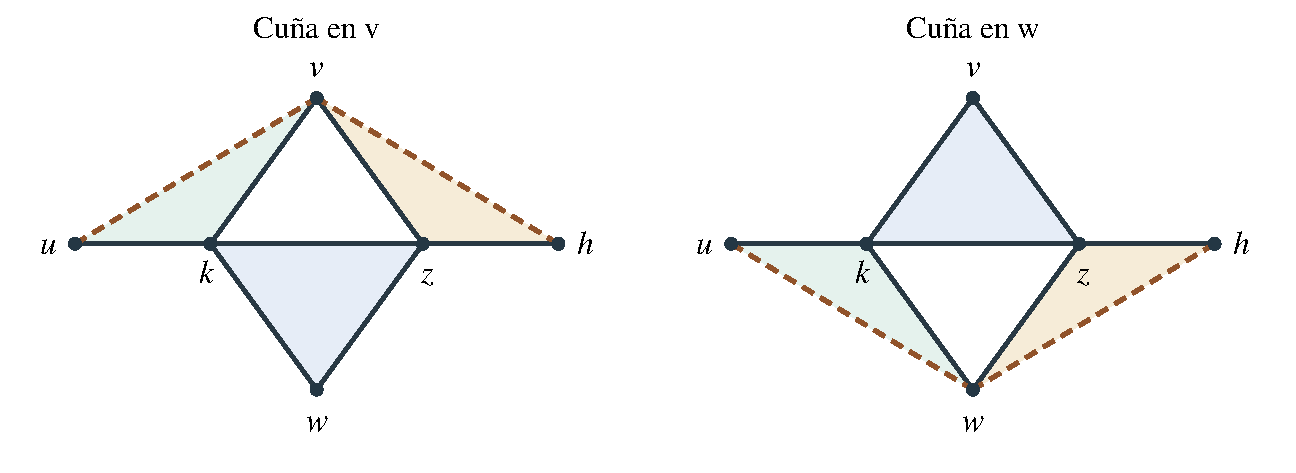
\includegraphics[width=.92\linewidth]{figures/crossing-hinge-es.pdf}
\caption{Las siete aristas continuas son las mismas en ambos paneles. Al añadir la cuña discontinua en $v$ se obtienen $kuv,hvz,kwz$. Al añadir la cuña discontinua en $w$ se obtienen $kuw,hwz,kvz$. Los tres triángulos sombreados en cada panel particionan las nueve aristas. La arista compartida $uh$ queda fuera de las dos descomposiciones.}
\end{figure}

\subsection{6. Demostración del teorema de estadísticas}\label{demostraciuxf3n-del-teorema-de-estaduxedsticas}

La misma asignación debe aproximar los conteos prescritos en todo el grafo y en su núcleo original. Elegimos las reservas de anfitriones antes del borrado de manera que cada Pasch se cuente en el bloque al que corresponden sus bases.

\textbf{Construcción de las reservas iniciales.} Usamos los dos órdenes del Lema 5 para los 54 tipos de rol. Para cada uno de los 66 tipos restantes tomamos un bloque aparte sobre el núcleo original, \(K_{t,t}\) para dos roles distintos y \(K_t\) para un solo rol, cada uno con \(Kt\) anfitriones. El núcleo original y estos dos conjuntos de anfitriones usan a lo sumo \([15+K(1296j+66)]t\) vértices. En la sección 4 sustituimos \(B_j\) por el factor entre corchetes. Su orden sigue siendo \(\Theta_p(j)\), así que aún se aplican la estimación de redondeo y (10).

Cada una de las tres clases de color tiene \(d_0=5t\) vértices originales. Sea \(w\) el mayor múltiplo de \(d_0\) a lo sumo \(p^2 n/64\), y tomemos \(|W|=w\). Como \(t=\Theta_p(n/\sqrt{\log n})\), tenemos \(w\sim p^2 n/64\). Dividimos los anfitriones restantes en cuatro reservas iguales, con a lo sumo tres anfitriones adicionales que solo son vecinos de \(W\). Cada reserva contiene al menos \(n/8\) anfitriones para \(n\) grande. Una solo es vecina de \(W\) y cada una de las otras tres es vecina de \(W\) y de una clase de color original. Como antes, todos los anfitriones originales también son vecinos de \(W\).

Partimos \(W\) en conjuntos de \(d_0\) vértices. En la reserva del color \(i\) designamos a cada conjunto \(\lceil(1+\eta)d_0/p\rceil\) anfitriones, distintos de los de los demás conjuntos, para su grafo \(K_{d_0,d_0}\) de solicitudes hacia \(V_i\). Se requieren \(((1+\eta)/p+o(1))w<n/8\) para \(\eta\) fijo y pequeño. Tomamos \(\lceil(1+\eta)w/p\rceil<n/8\) anfitriones de la cuarta reserva para el bloque terminal \(K_w\). En los bloques originales usamos la subreserva prescrita por el Teorema 1 dentro de los \(Kd\) anfitriones disponibles. Cuando dos pares de prefijos reutilizan una reserva en el Lema 5, la misma subreserva sirve a sus conjuntos disjuntos de vértices. Todas estas elecciones se hacen antes del borrado.

\textbf{Lema 7 (localización de las configuraciones de Pasch).} Con las reservas iniciales descritas, toda configuración de Pasch de los candidatos designados pertenece a exactamente un bloque auxiliar, restringiendo los bloques secundarios a las bases que les corresponden. La conclusión vale para cualquier subfamilia de candidatos, en particular para cualquier asignación posterior al borrado.

\emph{Demostración.} \emph{Bloques terminal y mixtos.} Cada uno de los cuatro triángulos tiene un anfitrión. Todo vértice de un Pasch aparece dos veces, de modo que las cuatro apariciones de anfitrión corresponden a exactamente dos anfitriones. Los dos triángulos de un mismo anfitrión tienen bases disjuntas, pues de otro modo compartirían una arista cruzada. Por tanto, los cuatro vértices del núcleo aparecen una vez en cada anfitrión. Los dos emparejamientos sobre estos cuatro vértices no comparten bases porque los triángulos de un Pasch son disjuntos en aristas. Su unión es un ciclo de longitud cuatro. Un anfitrión de un bloque mixto usa bases entre un conjunto de la partición de \(W\) y una clase \(V_i\). Si un segundo anfitrión usa los mismos cuatro vértices, debe pertenecer al mismo bloque mixto. Su emparejamiento alternativo vuelve a usar pares mixtos o necesitaría un anfitrión que sirviera a la vez un par interno a \(W\) y otro interno al núcleo original. Las asignaciones de los anfitriones excluyen esta segunda posibilidad. Un Pasch sobre cuatro vértices de \(W\) está en el bloque terminal.

\emph{Pares de roles originales.} En el núcleo original, un anfitrión que usa un rol repetido obliga a que los cuatro vértices pertenezcan a ese rol. Si hay dos roles distintos, un emparejamiento con dos pares internos exigiría que un anfitrión sirviera a ambos roles internamente. Por tanto, el segundo anfitrión debe servir al mismo par de roles que el primero. Para los 66 tipos, esto ya identifica el bloque.

\emph{Pares de roles que usan los dos órdenes.} Para uno de los otros 54 tipos escribimos las bases del primer anfitrión como \(u_1v_1,u_2v_2\) y las del segundo como \(u_1v_2,u_2v_1\). En cualquier coordenada que observa el primer anfitrión, la igualdad de las coordenadas de los puntos medios da \(u_1+v_1=u_2+v_2\). Las dos diferencias cruzadas coinciden y su valor común es el promedio de las dos diferencias directas. Si el primer anfitrión falla en una coordenada original anterior a la del segundo, (9), tras dividir por la distancia entre roles, sitúa la dirección cruzada fuera de \(S_m\). Ambas bases cruzadas retenidas deben estar dentro de \(S_m\) en cada coordenada original anterior a su fallo. Esto incluye la penúltima coordenada si el bloque es secundario. Por tanto, las coordenadas de fallo coinciden.

Los dos anfitriones observan ahora el mismo prefijo. Allí tenemos \(u_1+v_1=u_2+v_2\) y \(u_1+v_2=u_2+v_1\). Al restar obtenemos \(2(v_1-v_2)=0\). Como \(m\) es impar, coinciden los dos prefijos de \(v\) y los dos de \(u\). La dirección que falla determina la clase y el punto medio común fija el prefijo del centro. Los cuatro triángulos pertenecen al mismo bloque. El argumento usa solo la asignación de las bases a bloques y las incidencias inicialmente permitidas, por lo que se aplica tanto a un Pasch realizado como a un sumando de \(P_\lambda\). Cada base corresponde a un único bloque, así que el bloque común es único. \(\square\)

\emph{Demostración del Teorema 2.} El menor lado de un bloque original tiene tamaño al menos \(m^2\), y hay \(O(n^2)\) bloques no vacíos. Para \(\eta\) fijo, la probabilidad de que algún bloque incumpla el Teorema 1 es a lo sumo \(O(n^2)\exp(-\Omega_{p,\eta}(m^{2/3}))=o(1)\). En cada bloque que lo satisface elegimos los factores y los pesos positivos corregidos \(\mu\) del Teorema 1. Aplicamos T+ a cada bloque auxiliar completo. En un bloque secundario descartamos todo triángulo cuya base corresponde a un bloque primario, con lo que se retiran las dos incidencias cruzadas del triángulo del soporte secundario. Los triángulos conservados determinan el soporte final de ese bloque. En los demás bloques, cada incidencia seleccionada por los factores se usa exactamente una vez. Los bloques distintos con un anfitrión común tienen extremos del núcleo disjuntos, y cada base conservada pertenece a un único bloque. Obtenemos así una asignación completa. Las aristas cruzadas supervivientes fuera de su soporte seleccionado quedan disponibles como aristas individuales en el cálculo de la partición (7). La identidad (7) y el conteo de vecinos en \(W\) prueban (5) y (6) también para esta elección de testigos.

\textbf{Comparación del objetivo aleatorio con el prescrito.} Consideremos un bloque auxiliar completo de lado \(d\) y con una reserva prescrita de tamaño \(r\). Extendemos \(\mu\) por cero a los candidatos descartados y ponemos

\[\widetilde\lambda_T=\frac{\mathbf1_{\{\text{both incidences of }T\text{ survive}\}}}{p^2r}.\]

En los triángulos que conservan los factores, el peso inicial del Teorema 1 es \(1/a_h\) o \(1/(a_h-1)\). En ambos casos el denominador es \(d^2/r+O_p(1)\). Como \(pr/d=1+\eta+O_p(1/d)\), este peso inicial difiere de \(1/(p^2r)\) en \(O_p((\eta+1/d)/d)\). La corrección para obtener \(\mu\) es \(O_p((\eta+d^{-1/3})/d)\). Hay \(O_p(d^3)\) candidatos. Los factores descartan \(O_p(\eta d^2)\) incidencias supervivientes para \(d\) grande, cada una de ellas en \(O(d)\) candidatos de peso \(O_p(1/d)\). Por consiguiente

\[\sum_T|\mu_T-\widetilde\lambda_T|
     =O_p\big((\eta+d^{-1/3})d^2\big).
\tag{13}\]

Así queda acotado el cambio de objetivo para toda \(|f|\le1\). En el caso de Pasch, desarrollamos la diferencia de dos productos cambiando uno de sus cuatro factores cada vez. Un triángulo fijo pertenece a \(O_p(d^3)\) configuraciones candidatas (se eligen el segundo anfitrión y los dos vértices adicionales del núcleo), y cada uno de los otros tres pesos es \(O_p(1/d)\). Por tanto, una constante por (13) acota también el cambio del objetivo de Pasch.

La esperanza de \(\widetilde\lambda_T\) es \(1/r\). Los cuatro triángulos de un Pasch usan ocho aristas cruzadas distintas, así que la esperanza del producto de sus pesos de comparación es \(p^8/(p^2r)^4=r^{-4}\). De esta manera, (1) es la esperanza de cada objetivo de comparación. Cambiar una incidencia afecta a \(O(d)\) triángulos y \(O_p(d^4)\) configuraciones candidatas de Pasch, y modifica cualquiera de los dos objetivos en \(O_p(1)\). En el bloque hay \(O_p(d^2)\) ensayos independientes de incidencias. La desigualdad de diferencias acotadas {[}9{]} da una desviación de a lo sumo \(d^{5/3}\) salvo con probabilidad \(2\exp(-\Omega_p(d^{4/3}))\) por objetivo. Una cota de unión basta para todas las funciones de prueba y todos los bloques prescritos.

\textbf{El núcleo original.} Ponemos \(a=\lfloor j/2\rfloor\) y \(\rho_m=|S_m|/m^2\). La región que define \(S_m\) en {[}1, §6{]} excluye el cuadrado \([0,1/2)^2\). En la cuadrícula impar ese cuadrado contiene \(((m+1)/2)^2\) puntos, por lo que \(\rho_m\le 3/4\). Un bloque primario es temprano si su primer fallo ocurre en una coordenada \(i\le a\). Su lado tiene tamaño \(m^{2(j-i)}\ge\sqrt t\). Incluimos entre los bloques grandes los 66 tipos de rol sin restricciones. Estos bloques tienen lado \(t\) y se usan completos.

Para un par fijo de roles distintos, cada dirección aparece en exactamente \(t\) bases, una por posición de partida. En cada uno de los 54 tipos restringidos, los bloques tempranos contienen, por tanto, exactamente \(t^2(1-\rho_m^a)\) bases, cada una una sola vez. Los demás bloques primarios tienen a lo sumo \(t^2\rho_m^a\) bases. En el orden secundario, incluso \emph{antes} del recorte, las primeras \(j-2\) coordenadas originales deben satisfacer la condición. Por tanto, sus bloques completos tienen en total a lo sumo \(t^2\rho_m^{j-2}\) bases, pues la última coordenada y su clase determinan a lo sumo un bloque por base. Para \(j\ge4\), esto es a lo sumo \(t^2\rho_m^a\). Al sumar sobre los 54 tipos se obtiene la cota \(108t^2(3/4)^a=o(t^2)\) para las bases tardías y secundarias, contadas con multiplicidad.

En cada uno de estos bloques menores pedimos a T+ solo el conteo de Pasch, con precisión fija, por ejemplo uno. Hay \(O_p(d^6)\) configuraciones candidatas, cada una con peso fraccionario \(O_p(d^{-4})\) en la semilla, de modo que el conteo realizado es \(O_p(d^2)\). El objetivo inicial satisface la misma cota. El recorte reduce ambos conteos. Para una función de prueba de valor absoluto a lo sumo uno, cada base aporta a lo sumo una unidad en la asignación y en el objetivo inicial. Por el Lema 7, cada Pasch se contabiliza en un solo bloque. En conjunto, los bloques menores aportan \(o(t^2)\) a cada comparación, uniformemente en las funciones de prueba.

\textbf{Una elección conjunta de descomposiciones.} Aplicamos T+ en cada bloque temprano, sin restricciones, mixto y terminal a todas las restricciones de las funciones de prueba dadas y al conteo de Pasch conjuntamente. En estos bloques \(N\ge d\ge\sqrt t\). Así, para \(q\) fijo, tenemos \(n^q\le N^{2\lceil q\rceil+2}\) para \(n\) suficientemente grande, usando \(t=\Theta_p(n/\sqrt{\log n})\). La cota de concentración anterior vale a la vez para la cantidad polinómica de bloques y funciones de prueba. En ese suceso, la suma de los errores de comparación de objetivos y de descomposición en cada bloque de este tipo es a lo sumo \(O_p((\eta+\varepsilon+d^{-1/3})d^2)\) para \(\eta,\varepsilon\) fijos. Cada término se carga una vez a su bloque. Los bloques originales satisfacen \(\sum d^2=O(t^2)\) contando los bloques secundarios completos. Para toda la construcción, \(\sum d^2=O_p(n^2)\), pues un bloque completo contiene \(\Theta(d^2)\) bases. Al sumar primero en los bloques originales y luego en todos los bloques obtenemos errores normalizados \(O_p(\eta+\varepsilon)+o(1)\) en ambas escalas para la misma asignación.

Para obtener una única sucesión de testigos, tomamos \(\eta_i,\varepsilon_i\downarrow0\) que satisfacen el Teorema 1. En la etapa \(i\) admitimos hasta \(n^i\) funciones de prueba. Elegimos \(n_i\) creciente de modo que a partir de \(n_i\) los órdenes de los bloques relevantes superen los umbrales de T+, ambos errores normalizados restantes sean a lo sumo \(1/i\) y la probabilidad de fallo para cualquier familia dada de este tamaño sea a lo sumo \(1/i\). Las estimaciones dependen solo del número y de la cota uniforme de las funciones de prueba. Usamos las reservas de la etapa \(i\) para \(n_i\le n<n_{i+1}\). Todo \(q\) fijo queda cubierto a partir de alguna etapa. Los testigos y los pesos de referencia son independientes de la elección de las funciones de prueba. Una vez elegidas, sus objetivos se determinan antes del borrado. La asignación puede depender tanto de las funciones como del borrado. Así se demuestran (2) y (3).

\textbf{Los dos conteos de Pasch.} En un bloque bipartito, el número de ciclos de cuatro bases es \(\binom d2^2\). En un bloque clique es \(3\binom d4\). En cada ciclo, los dos emparejamientos alternados pueden recibir anfitriones distintos de \(r(r-1)\) maneras, cada una de peso \(r^{-4}\). Así, el objetivo inicial de Pasch por bloque es su número de ciclos de longitud cuatro multiplicado por \((r-1)/r^3\). Esto es \(O_p(d^2)\), una cantidad acotada por base. Hay \(O(t^2+wt)=o(n^2)\) bases originales y mixtas, incluso contando las copias auxiliares. La clique terminal aporta el término principal. Allí \(r\sim w/p\), por lo que

\[3\binom w4\frac{r-1}{r^3}
   =\frac{p^2w^2}{8}+o(n^2)
   =\frac{p^6}{32768}n^2+o(n^2).\]

En el núcleo original, los 105 pares de roles distintos se reparten en 51 tipos sin restricciones y 54 restringidos. Los bloques bipartitos grandes tienen en total \([51+54(1-\rho_m^a)]t^2=(105+o(1))t^2\) bases. Hay además 15 bloques clique sin restricciones de orden \(t\). Uniformemente en los bloques grandes, \(d\to\infty\) y \(r/d\to1/p\) a lo largo de la sucesión elegida. Así, \(\binom d2^2(r-1)/r^3=(p^2/4+o(1))d^2\) en un bloque bipartito y \(3\binom t4(r-1)/r^3=(p^2/8+o(1))t^2\) en cada bloque clique. Los bloques menores aportan \(o(t^2)\). La suma de los objetivos da \[P_{\lambda,U}=\left(105\,\frac{p^2}{4}+15\,\frac{p^2}{8}\right)t^2+o(t^2)
=\frac{225p^2}{8}t^2+o(t^2).\] Las ecuaciones (2) y (3) transfieren ambos conteos objetivo a \(\mathcal D\), lo que prueba (4). \(\square\)

A lo largo del artículo, \(p\) se mantiene fijo al crecer \(n\). El margen de masa de lista del Teorema 4 y las densidades de vecinos comunes del Teorema 1 se obtienen con \(p\) fijo. Para \(p=p(n)\) tendiendo a cero, queda determinar con qué rapidez puede decrecer \(p\) y aun conservarse una cota inferior del orden de (5) y una asignación completa tras el borrado con alta probabilidad.

\subsection{7. Formalización}\label{formalizaciuxf3n}

El suplemento de Lean 4 del 24 de noviembre de 2026 está disponible en \url{https://raw.githubusercontent.com/jtraverso/split-clique-partition-gap/main/preprints/SPLITGAPIII/05_formalization/split-gap-iii-lean-v0.4.zip}. La edición PDF incluye también el archivo como adjunto. Su SHA-256 es \nolinkurl{f5e51ff6a95f04688e92e5c291528ba14c689acda765282cde10c5a4c55cba46}. La tabla recoge las declaraciones principales del espacio de nombres \texttt{SplitGapIII}. El archivo incluye las fuentes, las dependencias fijadas y los informes de axiomas de 77 declaraciones. El umbral óptimo del Teorema 4, la construcción con alta probabilidad de un mismo soporte que satisface H1--H4 en el Teorema 1 y las estimaciones asintóticas a dos escalas del Teorema 2 se demuestran analíticamente en las secciones 2, 5 y 6, respectivamente.

{\def\LTcaptype{none} % do not increment counter
\begin{longtable}[]{@{}
  >{\raggedright\arraybackslash}p{(\linewidth - 2\tabcolsep) * \real{0.5000}}
  >{\raggedright\arraybackslash}p{(\linewidth - 2\tabcolsep) * \real{0.5000}}@{}}
\toprule\noalign{}
\begin{minipage}[b]{\linewidth}\raggedright
Declaración de Lean
\end{minipage} & \begin{minipage}[b]{\linewidth}\raggedright
Alcance
\end{minipage} \\
\midrule\noalign{}
\endhead
\bottomrule\noalign{}
\endlastfoot
\nolinkurl{split_gap_recovery_all_orders}, \nolinkurl{all_orders_error_tendsto_zero} & Recuperación de la brecha para todo orden suficientemente grande en la construcción con copias adicionales de anfitriones. \\
\nolinkurl{hosted_clique_deficit_mem}, \nolinkurl{selected_hinge_condition} & Corrección entera en el retículo de la clique seleccionada y verificación de H4 mediante conteos de completaciones ordenadas de seis vértices. \\
\nolinkurl{hosted_pasch_one_block} & Localización de un Pasch con anfitriones a partir del bloque asignado a cada uno de sus cuatro triángulos candidatos. \\
\nolinkurl{selected_decomposition_with_reference_targets} & Una descomposición de T+ para todas las funciones de prueba y el conteo de Pasch en un soporte seleccionado, dadas la semilla, las hipótesis físicas y las cotas de error respecto de los objetivos de referencia. \\
\end{longtable}
}

\subsection{Apéndice A. Demostración de la Proposición 6}\label{apuxe9ndice-a.-demostraciuxf3n-de-la-proposiciuxf3n-6}

\emph{Demostración.} Para cada uno de los 54 tipos de rol y cada coordenada \(i\) y clase \(C\), tomamos el cilindro de direcciones definido por \(u_i\in C\) y dejamos libres las demás coordenadas. Usamos dos anfitriones por centro con las vecindades del Lema 5. Para una coordenada de centro fija \(z_i\), se obtiene un grupo de \(2s\) anfitriones idénticos. Asignamos cada dirección requerida a la primera coordenada que falla, a su clase en esa coordenada y a la correspondiente coordenada del punto medio. Cada centro completo determina un emparejamiento, porque cada extremo determina el otro. Los \(s\) centros completos del grupo dan, por tanto, un grafo bipartito de solicitudes de grado máximo a lo sumo \(s\). Cada par conserva al menos \(2s-2\lfloor s/2\rfloor\ge s\) anfitriones comunes. El teorema de coloración de aristas por listas de Galvin {[}4{]} da una asignación propia. Para cada uno de los 66 tipos restantes reservamos \(2t\) anfitriones adyacentes a todos los vértices del rol o par de roles correspondiente, donde \(t=m^{2j}\). Cada par conserva al menos \(t\) anfitriones comunes, ya que \(s\le t\). Entre roles distintos se aplica Galvin y dentro de un rol usamos la cota \(\chi'_\ell(K_t)\le t\) de Häggkvist y Janssen {[}5{]}.

Con el núcleo original, estos grupos usan a lo sumo \((147+2592j)t\le(255+2880j)t\le n/25\) vértices por {[}1{]}. Como en {[}2, Proposición 6a{]}, añadimos \(W\) de tamaño \(w\) y tres familias de \(w+v\) anfitriones vecinos de \(W\cup V_i\). Esto usa a lo sumo \(n/25+4w+3v\le24n/25+4\) vértices. Quedan lugares para \(r\) anfitriones adicionales por familia. Los anfitriones del relleno final son vecinos solo de \(W\). También podemos hacer que cada anfitrión original sea vecino de \(W\).

Escribimos \(b=\lfloor(v+r)/2\rfloor\). Cada par mixto de \(W\) a \(V_i\) conserva al menos \(w+v+r-2b\ge w\) anfitriones comunes en su propia familia. Como \(w\ge v\), Galvin permite colorear allí los pares mixtos. En cada vértice de \(W\), estas tres coloraciones usan a lo sumo \(v\) anfitriones en total, uno por vértice original. Para un par dentro de \(W\), al descartar las incidencias ausentes y todos los anfitriones ya usados en algún extremo quedan al menos

\[3(w+v+r)-2b-2v\ \ge\ 3w+2r\ \ge\ w\]

anfitriones disponibles. La cota de listas para \(K_w\) completa la asignación. Por construcción, los pares originales, mixtos e internos usan incidencias cruzadas disjuntas, así que (7) se aplica antes y después del borrado. \(\square\)

\subsection{Apéndice B. Estimación de los cortes para los factores seleccionados}\label{apuxe9ndice-b.-estimaciuxf3n-de-los-cortes-para-los-factores-seleccionados}

En un lado del núcleo de tamaño \(d\), escribimos \(k=d\) para un bloque bipartito y \(k=d-1\) para un bloque clique. Los grados requeridos en el núcleo son \(k\) y los grados requeridos en los anfitriones suman \(kd\). Ponemos \(\bar a=kd/r\). En el caso bipartito, \(|a_h-\bar a|\le1\). En el caso de la clique, los dos enteros pares consecutivos que encierran la media dan \(|a_h-\bar a|\le2\) y permiten alcanzar el total prescrito, porque \(kd\) es par. En particular, \(a_{\min},a_{\max}=\Theta_p(d)\) para todo \(\eta\) fijo y suficientemente pequeño y \(d\) grande.

Sean \(x=|X|\), \(y=|Y|\) y \(b=\min(x,y)\). Sea \(T=kx+\sum_{h\in Y}a_h-kd\) la demanda del corte. Si \(T\le0\), el corte satisface automáticamente la condición. Si \(T>0\), al expresar la demanda en términos de \(Y\) y luego de su complemento obtenemos \[a_{\min}(r-y)<kx,\qquad k(d-x)<a_{\max}y .\] Por tanto, \(r-y\le C_px\) y \(d-x\le C_py\). Si \(b=x\), elegimos \(b\) vértices del núcleo y a lo sumo \(C_pb\) anfitriones omitidos. Si \(b=y\), elegimos \(b\) anfitriones y a lo sumo \(C_pb\) vértices omitidos del núcleo. El número de opciones en cada caso se acota por \((d+r+1)^{(C_p+1)b+2}\) mediante listas ordenadas que se completan con un símbolo en blanco. Además, \(\max(x,y)=\Omega_p(d)\) porque \(d\le x+C_py\). De aquí, \(xy=\Omega_p(db)\) y \(b\ge1\).

Escribimos \(u=x/d\) y \(v=y/r\). Las desviaciones de los \(a_h\) respecto de \(\bar a\) suman cero, de modo que \(|\sum_{h\in Y}(a_h-\bar a)|\le2\min(y,r-y)=O_p(b)\). Como \(pr\ge(1+\eta)d\ge(1+\eta)k\), al restar la demanda de la media binomial resulta \[pxy-T\ \ge\ kd(1-u)(1-v)+\eta kd\,uv-O_p(b).\] Aquí \(kd\,uv=(k/r)xy=\Theta_p(xy)\). Para \(\eta>0\) fijo, el término de redondeo es \(O_p(xy/d)\), por lo que la media supera la demanda al menos en una fracción positiva fija de \(pxy\) cuando \(d\) es grande. La desigualdad de Chernoff acota la probabilidad de que falle este corte por \(\exp(-c_{p,\eta}db)\). La probabilidad de algún fallo es a lo sumo \[\sum_{b=1}^{d}\exp\big(C'_pb\log d-c_{p,\eta}db\big)
       =\exp(-\Omega_{p,\eta}(d)).\] La misma cota vale en ambos lados de un bloque bipartito. Al tomar la unión de los dos sucesos de fallo, los dos factores pueden usar la misma sucesión prescrita de grados en los anfitriones.

\subsection{Agradecimientos}\label{agradecimientos}

El autor agradece profundamente a su esposa María Paz y a sus hijos Lucas, Juan Cristóbal, Francisca, Raimundo y Benjamín por su amor, paciencia y apoyo.

\subsection{Uso de inteligencia artificial y herramientas computacionales}\label{uso-de-inteligencia-artificial-y-herramientas-computacionales}

Se utilizaron Claude, de Anthropic, y ChatGPT/Codex, de OpenAI, para explorar y comprobar argumentos y preparar el manuscrito.

El autor es responsable de los argumentos, las citas, el código y la presentación. Ningún sistema de inteligencia artificial figura como autor.

\subsection{Referencias}\label{referencias}

{[}1{]} J. P. Traverso Gianini, \emph{Nearly Quadratic Additive Gaps for Edge-Clique Partitions of Split Graphs}, preprint 1.0 (2026), Lema 2.1 and §§4--6. \url{https://doi.org/10.5281/zenodo.24408988}

{[}2{]} J. P. Traverso Gianini, \emph{Stability of the Clique Partition Gap in Split Graphs}, preprint 1.0 (2026), Teorema 1, Lema 2 and Proposición 6a. \url{https://doi.org/10.5281/zenodo.24452724}

{[}3{]} M. Bonamy, M. Delcourt, R. Lang and L. Postle, \emph{Edge-colouring graphs with local list sizes}, Journal of Combinatorial Theory, Series B \textbf{165} (2024), Teorema 6. \url{https://doi.org/10.1016/j.jctb.2023.10.010}

{[}4{]} F. Galvin, \emph{The List Chromatic Index of a Bipartite Multigraph}, Journal of Combinatorial Theory, Series B \textbf{63} (1995), 153--158. \url{https://doi.org/10.1006/jctb.1995.1011}

{[}5{]} R. Häggkvist and J. Janssen, \emph{New bounds on the list-chromatic index of the complete graph and other simple graphs}, Combinatorics, Probability and Computing \textbf{6} (1997), 295--313, Teorema 1.1. \url{https://doi.org/10.1017/S0963548397002927}

{[}6{]} J. P. Traverso Gianini, \emph{Triangle decompositions III: Physical typed absorption and prescribed statistics}, preprint 1.0 (2026), Teoremas T y T+, §§2.1--2.3. \url{https://doi.org/10.5281/zenodo.23867836} \url{https://github.com/jtraverso/physical-typed-absorption}

{[}7{]} J. Balogh, J. He, R. A. Krueger, T. Nguyen and M. C. Wigal, \emph{Clique covers and decompositions of cliques of graphs}, Advances in Combinatorics (2026), Paper No.~9, Teorema 1.10. \url{https://doi.org/10.19086/aic.2026.9}

{[}8{]} V. Jain and H. T. Pham, \emph{Optimal thresholds for Latin squares, Steiner triple systems, and edge colorings}, Proceedings of the 2024 Annual ACM-SIAM Symposium on Discrete Algorithms, 1425--1436. \url{https://doi.org/10.1137/1.9781611977912.57}

{[}9{]} C. McDiarmid, \emph{On the method of bounded differences}, in \emph{Surveys in Combinatorics, 1989}, London Mathematical Society Lecture Note Series 141, Cambridge University Press (1989), 148--188. \url{https://doi.org/10.1017/CBO9781107359949.008}

{[}10{]} P. Keevash, \emph{The optimal edge-colouring threshold}, arXiv:2212.04397. \url{https://arxiv.org/abs/2212.04397}

\end{document}
